\documentclass{article}
\usepackage{natbib}
\usepackage{hyperref}
\usepackage{times}
\usepackage[section]{placeins}
\usepackage{gensymb} % How can I write a \textdegree~ (degree) symbol in LaTeX?
%\graphicspath{ {/Videography_figures}}

\newcommand{\BibTeX}{{\sc Bib}\TeX}

\title{Santa Ana Sucker Habitat Evaluation}
\author{C. Flynn, E. Harris-Tyrrell, O. Howie, L. Ho-Israel, S. Janssen, \\N. Larson, F. Lyles, W. Nore\~na, V. Sanchez-Jimenez, A. Vacas, D. Wagner,\\ Ed. Marc Los Huertos}
<<<<<<< HEAD
\IfFileExists{upquote.sty}{\usepackage{upquote}}{}
=======

\usepackage{Sweave}
>>>>>>> 718073c554b7ba0f274d172b3b3253ca947bb73b
\begin{document}
\Sconcordance{concordance:Report_DRAFT.tex:Report_DRAFT.Rnw:%
1 11 1 1 0 228 1 1 5 5 1 1 5 6 1 1 4 7 1 1 4 13 1 1 5 10 1 1 4 3 1 1 4 %
116 1}


\maketitle

\newpage
\tableofcontents
\newpage

\section{Introduction}

\subsection{Scope of Problem}

The Santa Ana sucker (\emph{Catostomus santaanae}) is a 16 cm fish that lives in the rivers of Southern California. The species has been listed as threatened by the US Fish and Wildlife Service, partially due to their losing over 70\% of their habitat \citep{obrien2011status, usfishandwildlifeservice14}. Also, in the 1960s, the habitat of the suckers would range from 10-26\textdegree~C \citep{greenfield70}.  This rise in temperature is most likely due to the extreme industrialization of the stream; much of it runs over concrete, which heats up to extreme temperatures in the sunlight.  A majority of the stream water also comes from discharge from a sewage treatment plant upstream, creating an unhealthy and unnatural environment.  The river discharge is also greatly diminished from what it used to be due to the extreme drought in Southern California.  The river is shallower, slower moving, and has less snow melt coming from the mountains, all of which factor into an increase in temperature. Biological Oxygen Demand (BOD) may also have deviated significantly from typical values in a less disturbed stream. 

As the Santa Ana Sucker's population has declined, the abundance of the red algae (\emph{Cosmopogen aeruginosus}) has risen significantly in the Santa Ana River. This may also be contributing to the sucker's decline, but the environmental variables that control the red algae's distribution in the Santa Ana River are currently not well understood. The direct effect this invasive algae has on \emph{C. santaanae} is also poorly constrained. 

In general, the environmental variables that influence \emph{C. santaanae} populations are poorly understood. Better understanding of water temperature, discharge rates, BOD, and red algae distribution could aid in conservation efforts of this federally endangered fish. 

\subsection{Problem Statement}

This project began with the broad driving question, "How can the Santa Ana sucker be saved?" To that end, we have tried to constrain what environmental variables affect \emph{C. santaanae} distributions to water temperatures, BOD, red algae content, etc. 

\subsection{Background (Literature Review)}

\textbf{[FOR NEXT PERSON WHO EDITS: Try to create a compelling reason why we sampled what we sampled... and set us up for the discussion section...]}


The range of the fish is of significant interest to efforts for its preservation. The current range of the Santa Ana Sucker differs significantly from its historic distribution in the Los Angeles Basin \citep{brown2005aquatic, saiki2007life}. The habitat value of the Santa Ana sucker is highly constrained by the reach of the Santa Ana river that we evaluated, where the water source is treated discharges for most of the year --- in this context the river reach is highly modified in terms of it's hydrology, geomorphology,  water quality, and habitat characteristics--- becoming a disconnected stream \citep{poole2002fluvial}. 

\subsubsection{Stream Hydrology and Geomorphology}

According to Evans et al. 2005 \citet{evans2005long} \textbf{[not sure if this is the correct citations!]}\footnote{I thing this is the BOD group, can someone take this one?}, temporary reduction of flow, such as that which can occur when the treatment plant which now largely supplies the river halts releases of the water which now largely maintains, can significantly reduce the amount of habitat for suckers. Just last month, the Center for Biological Diversity reported that "by halting water releases critical to maintaining surface flows of the Santa Ana River, the Rapid Infiltration and Extraction (RIX) treatment plant is stranding and killing threatened fish" \citep{REF}. 

Understanding the role of stream substrate can be important in restoring various fish populations. For example, restoration projects seemed to be failing to prevent the Chinook population from falling in the Merced River \citep{albertson13}. The installation of gravel augmentation in a reconfigured channel seemed to have little impact on the salmon, suggesting that other factors were catalyzing the fall of the species. By comparing the restored portion with other portions of the Merced river, food web characteristics and flow discharge seemed to produce the same results on the various life stages of the salmon. However, higher temperatures, less woody debris, and minimal riparian cover seemed to limit populations in the restored portions. Restoration efforts are then presented with an added challenge of ensuring that every aspect of the ecosystem is beneficial to the species, which demands more work toward temperature regulation and attempts to restore the river bank. To see how the Santa Ana sucker would react to similar conservation efforts would be interesting in discussions in attempting to determine solutions.

\subsection{Water Quality}

We used this source to determine preferred temperature for the Santa Ana Sucker and in general to inform ourselves more about the fish. Little research has been done on specific threats to the Santa Ana Sucker, but the document did point out possible threats arising from hydrological modification and urban development in general. The idea emerged that water coming out of a treatment plant could potentially be a threat under hydrological modification or urban development.

Regarding the importance of water temperature to the fish, Moyle postulates that the sucker prefers environments with cool water \citep{moyle2002inland}. Again, the temperature of the Santa Ana River has been rising to levels greater than the sucker could stand \citep{REF}. Other types of fish have been known to regulate their body temperatures by moving to different areas in their habitat throughout the day (Matthews Berg Azuma 1994). Temperature can play a signficant role fish behavior. For example, \citet{sadler1980effect} found discharge downstream of a impoundment altered fish populiaton densities as a result of temperature. Human activities can increase water temperature. Water-based organisms are sensitive to temperature change, especially young fish due to limited mobility. The effect of temperature on fish varies greatly depending on other conditions of the lake or river environment of the fish in question \citep{loshuertos16}. Heat, temperature, thermal energy, and heat capacity all slightly change how heat is measured in an ecosystem. Water in general has a high heat capacity, which indicates its high specific heat. Thus, aquatic systems therefore often retain their heat and are less susceptible to changes in temperature than non-aquatic systems. Inflows/mixing can have an effect on water temperature but it is often hard to detect due to thermal stratification mixing, seasonal change in temperature profile depth, and small volume inflow in terms of fraction of the lake volume. Temperature impacts many other features of water quality, which will be important to keep in mind going forward with the project. \citet{coulter2015fluctuating} explain how young Flathead Minnows exposed to warmer temperatures underwent a nondirectional sex reversal . This paper shows us how temperature can greatly affect fish and stress them out. 

In addition, evidence suggests that the RIX discharge waters affect the growth and development of the of mosquito fish (xxx) and the Santa Ana sucker \citep{jenkins2009effects}.

\subsubsection{Community Ecology}

For the Santa Ana River sucker habitat, a central threat is the invasive Red Algae that has been spreading with alacrity in areas where the fish are known to be, including the reach below the Rapid Infiltration and Extraction (RIX) Treatment plan (Palenscar).There are concerns that the algae may be one of the contributing factors to the sucker's decline. For example, one of the important features of the Santa Ana River for the sucker is the presence of coarse substrate, that is, gravel and cobble, as opposed to silt and sand \citep{thompson2010influence}. The sucker has adapted to feeding on the diatoms that tend to grow on the former. There is also evidence that some of the diatoms on which the sucker feeds may be able to grow on the algae (are epiphytic). 

Algae biomass can depend on a range of variables, both biotic and abiotic \citep{winkelmann2014top}. In general, diatom growth dominance has been associated with high quality sucker habitat \citep{REF}. 

New introductions of the red algae are not unique to the Santa Ana River \citep{vzakova2013new}.

This may lead to the sucker being in contact with the algae when feeding. If the sucker is ingesting the algae, this may constitute a factor to the Suckers decline. Of course, ingesting the algae is not a necessity to the fish being negatively impacted; the algae may also disrupt the fish's well-being in unknown ways. 

Some researchers suggest that algae may actually crowd out the diatoms on which, along with algae and detritus, the sucker feeds \citep{thompson2010influence}. The presence of the algae in the same area and on the same type of substrate as the fish could indicate competition for resources between the algae\textbf{[ and the sh???]}\footnote{I am not sure where this was going\ldots}


\subsection{Objectives}
This experiment explores sevreal aspects of \emph{C. santaanae} habitat and distribution. Using measurments of river water temperature, overhead tree canopy cover, and sediment type we explore the environmental variables of the river and their relationship with the distribution of red algae. Our second goal of this study is to discover whether or not the Santa Ana suckers are coping with this dramatic increase in temperature by moving to cooler sections of the stream throughout the day, by recording video footage of \emph{C. santaanae} movement. 

Our goal with this experiment was to find out whether or not temperature was affecting the population and/or livelihood of the Santa Ana Sucker in the Santa Ana River.

Our goal is to obtain footage clearly showing the density of Santa Ana suckers in the different locations at different points in the day.  We hope to get accurate enough footage to count the number of fish in each video, then run an ANOVA test on each location to see if the quantity of fish significantly varies at different times of the day.  If they do, we will be able to conclude that the suckers move throughout the day to find their preferred temperature.

Does the Santa Ana Sucker shift its distribution in the Santa Ana River based on natural temperature changes that occur throughout the day? We believe that if we monitor the relative distribution of the Santa Ana Suckers throughout the day we will see a difference in sucker abundance between an upstream and downstream location in response to changing temperature throughout a 24-hour period.

Finally, this report aims to determine whether Biochemical Oxygen Demand (BOD) and water flow velocity are relevant to future research regarding the endangered Santa Ana sucker \emph{C. santaanae}. We collected water quality data from the Santa Ana River to answer the following questions: \emph{Do BOD levels vary in different sections of the river}; \emph{Do differing BOD levels correlate with the abundance of individuals?}; and \emph{Do the water flow rates in different sections of the river correlate with sucker populations?} Because the section of the river we evaluated regularly receives discharge water from a nearby water treatment facility, we believe that BOD levels will be relatively low, around 10 mg/L, decreasing further from the discharge point. Where the BOD levels are lower, we expect higher fish count. We also hypothesize that larger populations of the sucker will concentrate near high-flow sections. Through this experiment, we aim to inform Santa Ana sucker conservation efforts and hope to inform action by the nearby water treatment facility. 

The presence of the non-native red algae in the Santa Ana River and the possible relationship it holds with Santa Ana Sucker's decline. In the last five years, the non-native tropical red algae Cosmopogen Aeruginosus has been found in large quantities in the Santa Ana River. Using measurements of river water temperature, overhead tree canopy cover, and sediment type, we explore the connection these aspects of the river and their relationship with the red algae.

\begin{quote}
Our null hypotheses are H0: Water flow velocity and/or BOD levels do not significantly correlate with prevalence of the Santa Ana Sucker.
\end{quote}
\begin{quote}
Our alternative hypotheses are H1: Water flow velocity and/or BOD levels significantly correlate with prevalence of the Santa Ana Sucker.
\end{quote}
If we can reject one or both of our null hypotheses, we can conclude that the study of Biological Oxygen Demand (BOD) and water flow velocity are relevant to future conservation research for the endangered Santa Ana sucker \emph{C. santaanae}.


\section{Methods}

\subsection{Materials and Equipment}
\begin{itemize}
\item 2 Waterproof GoPro Hero 4 Silver cameras with mounts
\item 4 64GB microSD SanDisk memory cards
\item 4 Waterproof Re-Fuel 6-Hour ActionPack Battery for GoPro HERO by DigiPower
\item 2 HOBO Tidbit water temperature data loggers
\item 2 Grey Cinder block cubes open on two parallel sides, ~8in x 8in x 8in, Home Depot
\item 2 Grey Cinder block backs, ~8in x 8in
\item 1 bottle of Original Sticks to Everything Gorilla Glue
\item 4 HOBO Tidbit Water Temperature Data Logger,
\item 1 Optic USB U-4 Base Station with coupler and HOBOware software,
\item 4 Green Garden stakes to hold loggers in stream channel
\item Red flags,
\item Yellow marking tape,
\item Ice Bath for calibrating loggers
\item GPS Spherical Canopy Densiometer
\item 30cm x 30cm PCV Quadrat
\item Analog Thermometer
\item 10 m tapemeasure
\item Field Book Recording material
\item Computer, RStudio Server, Microsoft Exc
\item snorkleing goggles 

\end{itemize}

\subsection{Site Description}

We collected our video on-site at the Santa Ana River. As a class we chose to collect data from four points along a small stretch of the river that was easily accessible by car. Because of this, the part of the river we took data from was relatively close to roadways and traffic. 

The specific sites for our project consisted of one upstream location (site 2) and one downstream location (site 4), located roughly one kilometer apart. Site 2 was located just below the Rialto concrete channel and site 4 was a plunge pool. The upstream location was significantly more encumbered with large debris like rocks and branches. The downstream location was smooth and flat, with a bed of pebbles and smaller coarse sediments (Figure \ref{SAR_Image}). 

We evaluated the Santa Ana River between... near Colton, California (Figure \ref{SAR_Image}). 

This data was collected at three reaches in the Rialto portion of the Santa Ana river near Colton, California (Figure \ref{SAR_Image}). 

\begin{table}
\caption{caption}
\begin{tabular}{llll}\hline
Location & Latitude             & Longitude   & Description \\ \hline\hline
Site 1  &    &   & Rialto Channel \\
Site 2  & 34\textdegree 2'29"N          & 117\textdegree 21'15"W   & Above RIX Influx \\
Site 3  & 34\textdegree 2'21"N          & 117\textdegree 21'20"W   & Below RIX Influx\\
Site 4  & 34\textdegree 2'5"N           & 117\textdegree 21"17"W   & Pool, approximately 40-50 cm in depth\\ \hline
\end{tabular}
\end{table}

Site 4 was the plunge pool, located the furthest downstream. Site 3 was below the confluence and Site 2 was upstream from the confluence. 

The river was surrounded by a derelict lot filled with trash. It was very industrial, with many trucks idling by the roadside and industrial shipping buildings. Rip-rap to protect the channel levy. The area we walked through to approach the river was very sandy, with tire tracks. The river itself had some trash in it and was smaller than expected in contrast to rivers in other areas of the country, like the Pacific Northwest. 

Each observation contains the following variables: algae \% cover, canopy cover, water temperature, bed composition.  


\begin{figure}[!ht]
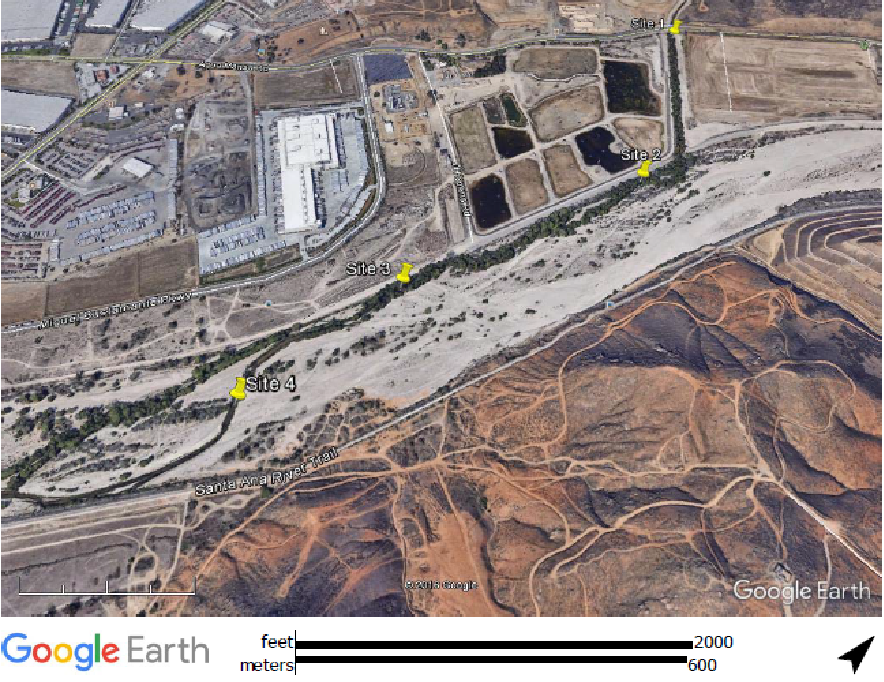
\includegraphics[width=1.00\textwidth]{Figures/SiteMap}
\caption{Google Earth --Example of a map. Needs a caption.}
\label{SAR_Image}
\end{figure}

\subsection{Habitat Evaluation}

The collection of data on the algae abundance, sediment type, and vegetation canopy cover of the Santa Ana River was done along the section of the river described in the site description section on September 20th, 2016, from 1pm to 3:30pm.

Temperature collection occurred from September 25th til October 1st for Site 2, and September 25th til October 4th for Sites 1, 3, and 4, every 15 minutes.

We evaluated 9 parameters from Sites 2-4, for a total of 27 measurements. At each site, beginning at Site 4, the following procedures were followed: 

\begin{enumerate}
\item A spot was chosen along the right bank. Each of the parameters were then measured.
\item For estimating algae abundance, we placed the 30  x 30 cm quadrat above the river bed and estimated the \% that was covered by algae to the nearest 10 \%.

\item The sediment type of the site was characterized as either fine or coarse based on the grain size of the 30x30cm section of stream bed covered by the quadrat as either fine or coarse. Coarse substrate was classified as anything larger than pebbles or sand, that is, larger than 6.5cm. If more than half of the area covered by the quadrat was coarse substrate, or fine substrate, the area was characterized as such respectively.

\item Canopy cover was measured from the same position as the algae by holding spherical canopy densiometer above water at elbow's length. Based on how many of the 15 intersections on the densiometer reflected overhead canopy, cover was then quantified on a 0-15 scale, 0 being the no canopy cover and 15 being full cover.

\item To measure temperature, we submerged the analog thermometer underwater and recorded the temperature in degrees Celsius.

\item Qualitative aspects of the river, such as presence of a pool or of logs, were also noted at each measurement spot.

\item Each measurement was then also taken at the middle of the river and the left bank of the cross-section. 

\item Steps above were repeated at two cross-sections between 0 and 10 meters downstream both chosen using a random number generator for a total of 3 cross-sections along a possible total length of 20 meters, and 3 measurements at each cross-section, for a total of 9 measurements per site. 
\end{enumerate}

At each of the corresponding water sample collection sites, water velocity was also measured using a SonTek FlowTracker Handheld Advanced probe, which emits sonar waves at a certain depth in the water column, and based on the feedback (20 pings) gives a velocity reading. Ideally, multiple readings would be taken at each site, after the probe is placed on a flat section of the riverbed where water appears to be flowing net in the same direction. 

\subsection{Videography}

We acquired all the necessary equipment for an underwater filming project, keeping in mind the length of time we wanted to keep our cameras underwater. We chose the GoPro Hero 4 Silver because of its battery life and recording time. We also considered safety and theft prevention for the cameras, and for this reason decided to mount the cameras in cube-shaped cinderblock structures with one open side that we constructed ourselves. In the lab, we set up all the equipment, built the cinderblock structures, and prepared everything for the field. Once in the field, we selected appropriate data sites, set up our cameras, and placed them at certain specific times of the day. More detailed information on these processes can be found in the following sections.

\subsection{Temperature Loggers}
We obtained four HOBO Tidbit water temperature Data Loggers to set up at the Rialto Channel at Agua Mansa (site 4), another at the point where the other discharge site meets the river (site 2), another just above that site (site 3), and a fourth in the pool where Suckers have previously been observed (site 1). Before going to the river, we programmed the loggers via our base station and the HOBOware software to collect water temperature data every 15 minutes. In order to start the data process, we put each logger into the coupler and pushed the level til the light was flashing. We then put them in the river by looping a garden stake through one, sticking it into the substrate, and securing it with rocks. We then put yellow marking tape on plants nearby and red flags along the bank to show where we left the main path. We repeated this for each site, making sure the loggers were secure and fairly hidden. After seven nights (for site 3) and eleven nights (for the other sites), we returned to the river and collected the loggers. In the lab, using the software, we loaded our data and transferred it to RStudio. Later, to calibrate the loggers, we put them in an ice bath for 6 minutes to ensure that the temperature settled around zero and each logger was measuring to the same temperature with the same accuracy.

\subsection{BOD Methods}

Approximately 1L of source river water was collected at each of two sites, one upstream location (site 2) closer to the wastewater discharge facility, and one downstream location (site 4). Ideally, these would be transported to the laboratory for analysis within four hours. BOD was carried out using the following methods...\textbf{[need to add method to report.bib]}

\subsection{Statistical Methods}

Using the R programming environment \citep{CRAN}, we use linear regression and ANOVA to analyze stream habitat variables. We also tested habitat value with fish count data comparing morning to afternoon counts. However, we acknowledge the fish count data are spatially and temporally autocorrelated, thus, our conclusions we make are serverely constrained based on the sampling methods.

\section{Results}


\subsection{Hydrology, Geomorphology, Canopy and Algae}

\textbf{[Velocity Measurements HERE]}

The the percent cover of the invasive algae may be influence by the stream substrate size (Figure \ref{fig:algae}, Panel A, p = 0.0643). We found no relationship between the percent cover of the invasive algae species on the canopy cover (Figure \ref{fig:algae} Panel B, p = 0.334).

\begin{figure}[!ht]
\caption{Algae abundance as a function of the bed composition (Panel A), where course sediments = 1 and fine sediments = 0 and canopy cover (Panel B).}
\label{fig:algae}
\end{figure}

As a control\footnote{I am not sure what this means?}, we also analyzed to what extend Site alone could predict Algae Abundance(Figure \ref{fig:algaesite}). Our ANOVA test yielded p-value: 0.008176 \textbf{which means the reach of the river studied is alone one of our best predictors of algae abundance, second only to temperature variation.}\footnote{this a discussion point, not a result.} 

\begin{figure}[!ht]
\caption{Algae Abundance as a function of Site.}
\label{fig:algaesite}
\end{figure}

The initial temperature data collected with an analog thermometer did not adequately describe the stream temperatures, so we relied on the temperature logger data for most of our analyses. We found that temperature fluctuated between a minimum of 25.12 degrees Celsius and a maximum of 31.37 degrees Celsius, which are all well above the 22 degrees that many studies found is the optimal temperature for the fish. The plunge pool, site 4, contained the most data points around 27.5 degrees, which proved true for each locations, having the most repetitive temperature between 27 and 28 degrees. Site 4, however, had the least temperature range, only varying between 27 and 28.5 degrees, while other sites tended to have a bigger variation, with site 1 varying up to 5.41 degrees. (Figures \ref{fig:Temp} and \ref{fig:tempbox}).

\begin{figure}[!ht]
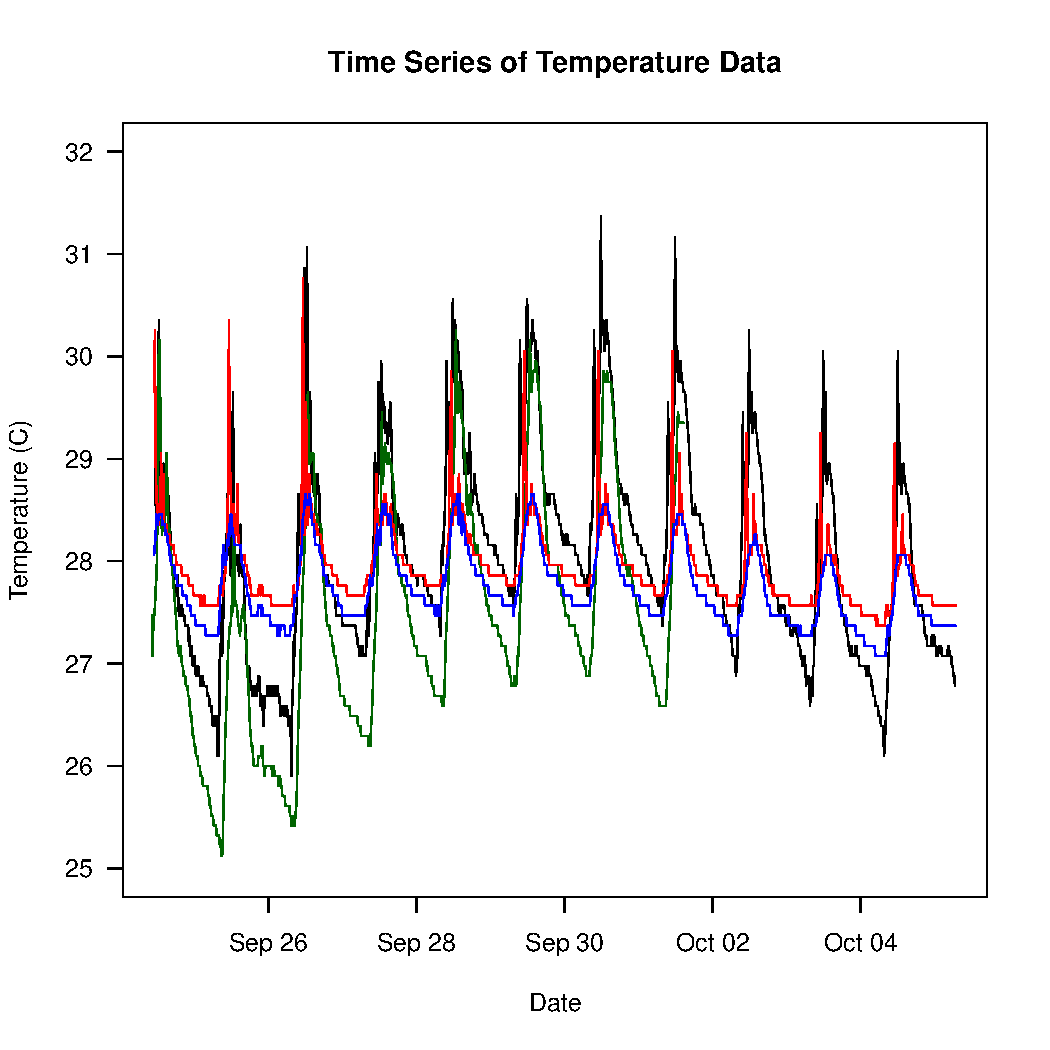
\includegraphics[width=0.90\textwidth]{Figures/Temp}
\caption{Temperature vs. time for all sites}
\label{fig:Temp}
\end{figure}
\begin{figure}
\label{fig:tempbox}
\caption{Box plots of temperature collected}
\end{figure}

We evaluated the relationship between algae abundance as a function of range of temperature (*C) experienced at each site (Figure \ref{fig:tempalgae}) \textbf{and found... what???}. While using our absolute temperature data as a predictor of algae abundance yielded p-value: 0.446 (cannot reject null hypothesis), using the other teams's temperature d range data yeilded \textbf{the much better p-value of 3.49e-05}\footnote{better?!!! says who?}. There is a strong nonrandom relationship between the range of temperatures a site experiences and the abundance of algae. However, with an Adjusted R-squared of only 0.4826\footnote{This is quite high in ecology, please revise}, there are clearly other important variables at work as well. We find that higher variation in water temperatures generally coorelates to higher algae abundance. 
\begin{figure}[!ht]
\caption{Ths is caption that needs info...}
\label{fig:tempalgae}
\end{figure}

\subsection{$BOD_5$ and Water Velocity}
Analysis of the data using quality control parameters indicated that two source water samples met minimum DO depletion standards. Our $BOD_5$ calculations of these data yielded the values:

\subitem Site 2 $BOD_5$= 22.1 mg/L 
\subitem Site 4 $BOD_5$= 27.3 mg/L 
<<<<<<< HEAD

The average recorded water flow velocities were:

\subitem Site 2: 0.27 ft/sec
\subitem Site 4: 1.09 ft/sec 
=======
>>>>>>> 718073c554b7ba0f274d172b3b3253ca947bb73b

The average recorded water flow velocities were:

\subitem Site 2: 0.27 ft/sec
\subitem Site 4: 1.09 ft/sec 

\subsection{Fish Counts}


At the upstream location (Site 2), no suckers were observed in the morning while one sucker occasionally swim out from behind a rock. At the downstream locatin (Site 4), we observed numeous fish \ldots (Table \ref{tab:fishcounts}). We counted an average of 20.1 suckers in the morning with a standard deviation of 6.0 fish.  In the afternoon, we counted an average of 32.2 with a standard deviation of 9.9, meaning both the average and the variance were higher in the afternoon.  The river was 27.8\textdegree C in the morning and increased to 28.4\textdegree C in the afternoon.  We calculated a p-value of 6.027e-13, which is less than .05 so we can reject our null hypothesis that tie of day will have no effect on the number of fish.

\begin{table}
\caption{Summary Statistics for Videography Fish Counts}
%\begin{tabular}{ |p{1.5cm}||p{1cm}|p{1cm}|{p2cm}|{p2cm}|{p2cm}|{p2cm}|{p2cm}|  }
\begin{tabular}{cccccccc}
 \hline
 \multicolumn{8}{c}{Videography Summary Statistics} \\
 \hline
 Section & Min & Max & Mean & Median & 1st Quartile & 3rd Quartile & K\\
 \hline
 Morning & 7 & 29 & 20.13 & 22  & 16.75 & 25 & -0.6\\
 Afternoon & 14 & 49 & 32.25 & 31 & 24.75 &  42 & -1.3\\
 \hline
\end{tabular}
\label{tab:fishcounts}
\end{table}

\textbf{[Text to describe Figure \ref{fig:fishsection}]}

\begin{figure}[!ht]
\caption{needs a caption! Can we change after to afternoon...}
\label{fig:fishsection}
\end{figure}


\textbf{[Text to describe Figure \ref{fig:reallygoodcrop}]}

\begin{figure}
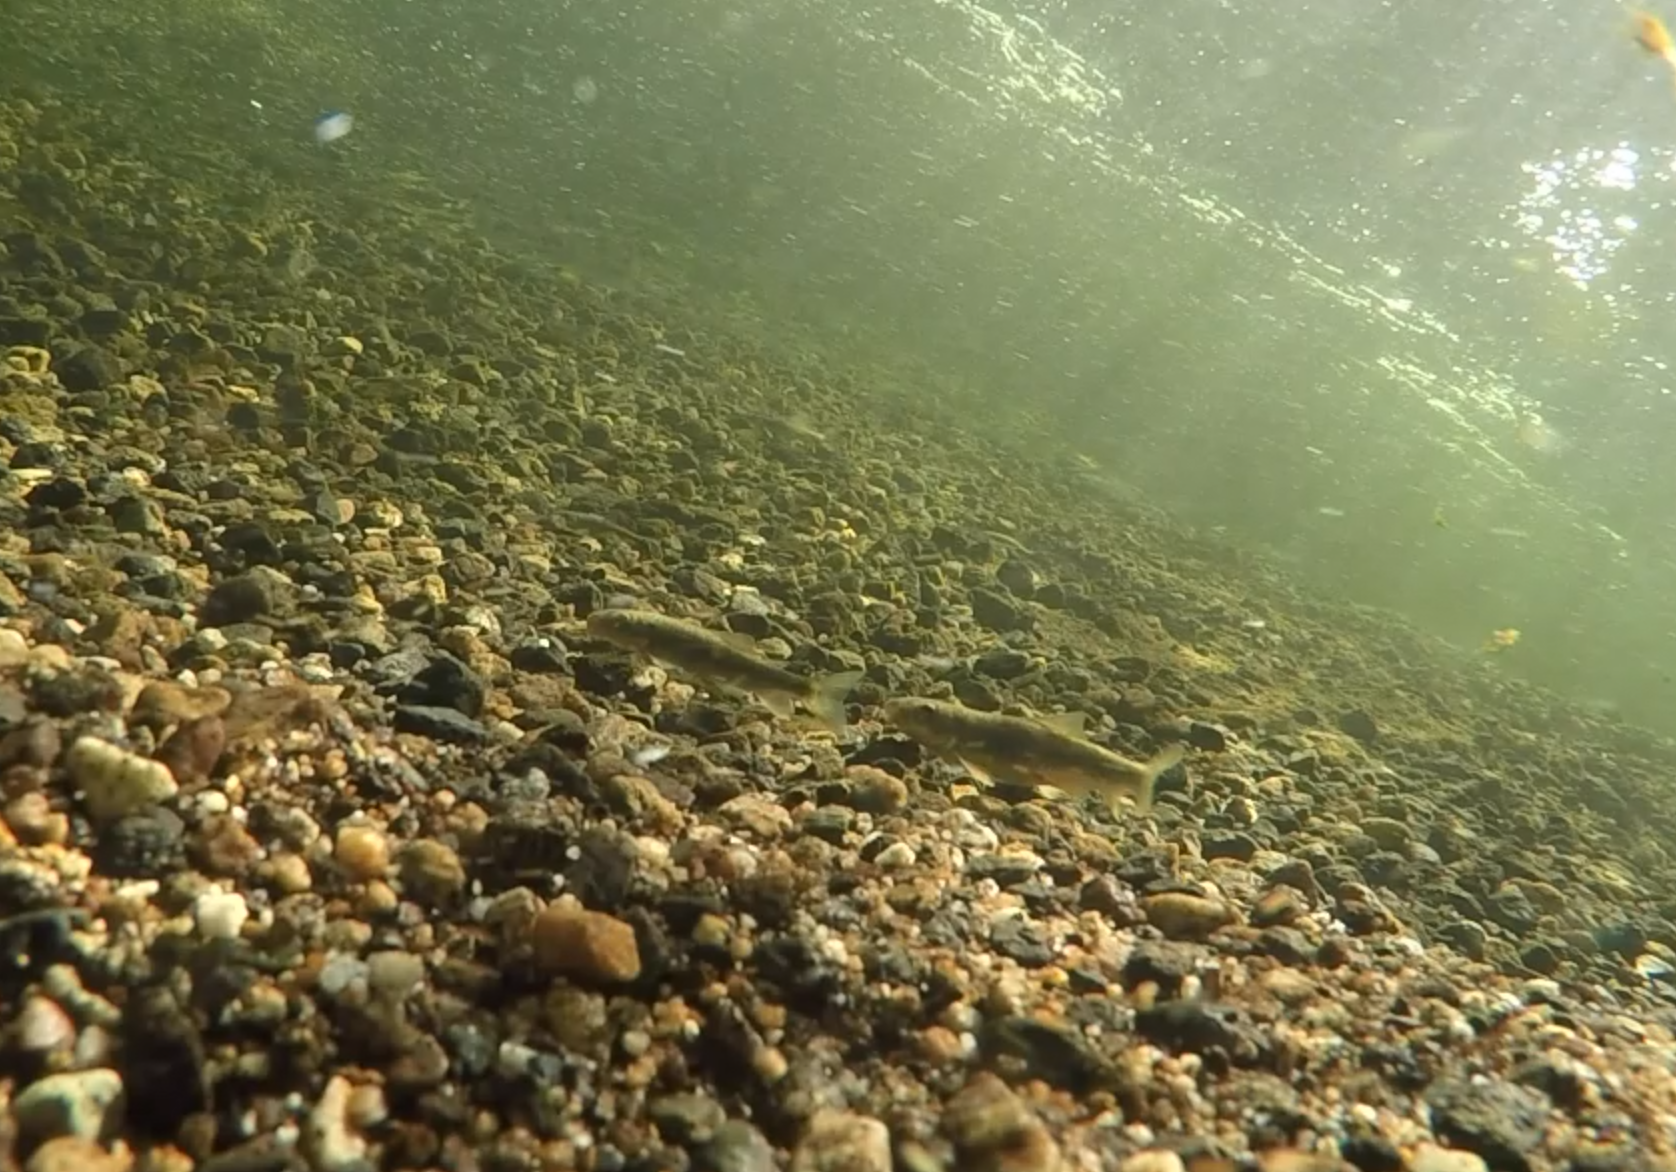
\includegraphics[scale=.4]{Videography_figures/reallygoodcrop}
\caption{A close up of a Santa Ana Sucker from the footage we collected.}
\label{fig:reallygoodcrop}
\end{figure}

\section{Discussion}

\subsection{Habitat Quality and Fish Activity}

\textbf{We need to describe the habitat value that we determined! relative to the literature...}

\subsubsection{Hydrology and Geomorphology and Algae?}

There is a statistically significant variation of algae abundance between the 3 sites examined in our study. Some measurements showed up to 100\% algae cover, while others exhibited none. This variation suggests the possibility that algae may be controlled by specific variables. We tested whether water temperature, water temperature variation, canopy cover, or stream bed composition could explain these variations. Of these possible causal factors, we found the strongest evidence for higher water temperature variation exerting a positive effect of algae abundance. The relationship between algae cover and streambed sediment composition of the stream bed was not statistically significant at the 95 \% level, but did tentatively suggest that algae may prefer coarse sediment. Red Algae in the Santa Ana River has a highly unequal distribution, that appears to be controlled in part by water temperature variation, with a possible small contribution of streambed sediment composition. 
Our exploratory study is one of the first to examine what variables may control red algae's distribution in the Santa Ana River. 

This indicates that there is probably some relationship between algae cover and sediment composition of the stream bed, and this should be examined in future. In general, alage seem to perhaps prefer coarser sediment. 

Future studies should more systematically examine the relationship between temporal variability in water temperature and algae abundance. Sediment type should be assigned to narrow categories such as silt, sand, gravel, and cobbles rather than simply being tagged as fine or coarse. More than 3 reaches/sites should be used. 

Most importantly, red algae's co-occurrence with the federally endangered Santa Ana sucker should be examined. These improvements on our experiment will yield a much better idea of what factors control red algae's distribution in the Santa Ana River, and create a statistically supported foundation for considering the algae's effect on Santa Ana Suckers.

\subsubsection{Temperature and Invasive Algae}

The temperature data include spikes on a daily basis, which were especially significant Sites 1 and 2. For example, Site 1 fluctuated up to 5.4 \textdegree~C a day. Our original hypothesis when we saw this was to assume water spikes were occurring from the Rialto Channel and as they travelled down river, becoming less extreme. In additioin, we did not find a temperature spikes traveling downstream. In fact, the spikes further downstream were actually occurring before the spikes upstream. We are unsure why there were such fluctuations in the river, because it did not appear that spikes were travelling downstream, based on the times that high and low temperatures occurred at different points in the river. 

\textbf{[NEED DISCUSSION COMPARING TEMPERATURE WITH LITERATURE...]}

\subsubsection{Fish Behavior and Counts}

In terms of fish population, using the data from the Fish and Wildlife Service, as well as the data from Clare and Wendy's group, we realized that there were no fish counted at site 1, only one fish counted in the afternoon at site 2 at various points, no fish were found by the FWS at site 3, but many fish were observed by Clare and Wendy in the plunge pool at site 4. Also, from previous results, we knew that most Santa Ana Suckers live in the plunge pool and prefer it there. This could be because of reasons other than temperature, but we did notice that there were less extreme spikes in site 4. Our videos of site 2 contained very few fish. 

This could be because the temperature further upstream was too hot for the suckers to live in; the temperature data found that at that location the water was between 30.25\textdegree~C in the afternoon and 25.12\textdegree~C in the morning. This is a range of 5.13\textdegree~C, which is a much larger range than the range found at site 4, where more suckers were found. In general, the fish were more abundant downstream, where the least extreme temperature spikes were occurring. From what we observed, the extreme temperature spikes at sites 1 and 2, and the medium spike at site 3, could have caused the fish to prefer to stay at site 4, where they are most abundant. This disproves our null hypothesis that the fish would be randomly spread throughout the channel and that temperature would remain fairly constant throughout the river, which suggests there could be a correlation between what is happening temperature wise and with the location of the suckers.

Also, the hottest temperatures that occurred at site 2 were almost at mortality rate for suckers, and were 1.59\textdegree~C higher than any temperatures found in site 4. It is possible that the fish prefer site 4 for other reasons than temperature, but correlations between temperature and Sucker abundance should be further explored.

When we compared the number of fish downstream in the afternoon compared to the morning, we had a p-value of 6.027e-13, meaning there were significantly more suckers in the afternoon than there were in the morning.  This suggests that the suckers do move downstream throughout the day to get to cooler temperatures.  On the afternoon we tested, the plunge pool (downstream) was 28.5\textdegree~C, whereas the river at our upstream location, closer to the concrete, was 29.4\textdegree~C. Throughout our longer term temperature testing, we noticed there was significantly more variation in temperature the further upstream we tested. These large temperature spikes and variability could have prevented fish from successfully habitating the upstream sites. 





We collected our data in a simple yet straightforward manner to ensure its comprehensibility and communicability. Not only does our data span over a week, 24 hours a day, but we collected at four different sites every 15 minutes, giving us a significant spread of data to work with. Given the limited timeline of the experiment, our data can be said to have captured a glimpse into an average week for this portion of the river, and can be used as a baseline and reference for future projects. A weakness was that we were not able to measure possible temperature stratification, since we only measured at one point for each of the four sites. 

Our data itself has left us with many unknowns. The water temperature measurements seem to fluctuate but not necessarily with the air temperature measurements, averaged, from that day. Compared with the historic averages, the week of our experiment was particularly hot, but the effect on the suckers is hard to determine as the air temperature data was not collected every fifteen minutes or even hourly (as our data was), and instead we had to rely on daily highs and lows. 

There were also pretty extreme spikes, but not occurring at times that suggested spikes were travelling downstream, originating from the Veolia water plant. Initially, Veolia agreed to send over their data on both the influx and outflux water temperatures, to allow us to see what was happening to water temperature from the plant. However, after a week of following up, we have not been able to get the data, as the CPO has hesitated to release it and says it will take up to a month to compile it. Without this data, it is hard to explain these randomly occurring spikes at different points in the river. This part of the data could have also been affected by canopy cover or stratification. 

It is difficult to determine if the temperature spikes were what caused the fish to choose to reside primarily in site 4, because there are a myriad of other variables. Other variables that could have affected where the fish chose to live include algae/food source, canopy cover, depth, or sediment type/size. What we do know is that the further upstream locations not only had a wide range of temperatures, but also experienced hotter temperatures than site 4, which was where the fish live. From our background research, we know that the US Fish and Wildlife Service found that Santa Ana Suckers prefer water that is around 22 degrees Celsius. None of our sites had water this cold, but site 4 had the least variability and averaged around 28 degrees. According to a brief overview from Larry Brown of the US Geological Survey, there are no fish at site 1, and at sites 2 and 3 there are only a few European chubs. At site 4 they estimated large numbers of fish but did not conduct a formal survey of this site. However, our video data showed a much larger population in the plunge pool. These population estimates were the results of random surveying, and could be limited in their applicability because of variation in site location and scope. For example, Larry Brown measured sucker populations in the Rialto drainage but not in the pool below it, which is where we placed our data logger. Therefore, it is difficult to tell to what extent the US Geological Survey’s data works with our data. 

\subsection{$BOD_5$ and Water Velocity}
Future study of dissolved oxygen levels and water velocity in the Santa Ana River measure any correlations with the recent Fish and Wildlife Service electroshock population data. Though we did not have access to this data, we had access to a rough estimate of the Sucker population from video-counting. In a week, about 12 fish were counted at Site 2 and 671 fish at Site 4. So, many more fish were spotted where the river velocity was higher and where the $BOD_5$ levels were higher. Since BOD can be less than 2 mg/L in clear water and reach hundreds of mg/L in organic waste water, a difference of about 5 mg/L between Site 2 and Site 4 is very small. It is unlikely a threshhold was reached between 22.1 and 27.3 mg/L that made Site 2 unliveable for the sucker. The difference in velocity is more significant and also supports the referenced existing literature that says water flow velocity is one of the primary determinants of sucker population. We recommend future research on the Santa Ana Sucker population focus on water velocity.

\subsection{Research Limitations}

Because of our experiemental design, it is unfortunately impossible to control by site for temperature variation and see if the relationship remains robust. This should be examined in future work. For videography, we did not formulate a standardized method with which to place our cameras in the water. For this reason, there were differences in footage from morning to afternoon as well as from site to site. For future studies, we recommend including physical place-markers in the river for the cinderblock structures, maybe in the form of flags placed directly in the river bed. Markers inside of the cinderblock structure that delineate the exact position and angle of the cameras would also be ideal in order to ensure the same exact field of vision is present throughout the collected footage. 

Due to the learning curve associated with performing the $BOD_5$ experiment for the first time, procedural complications were encountered at several points in the experiment. As a result, initial DO content was not measured for the source water samples before incubation. We estimated a constant initial sample DO measurement using the DO of the seeded blanks. This decreased the accuracy of the BOD5 calculations, but gave a relative idea of the initial values. Inconsistent DO measuring methods also added to the inaccuracy of the final BOD5 results. Despite these procedural errors, our BOD5 measurements, 27.3493 mg/L at Site 4 and 22.069 mg/L at Site 2, did reach quality control parameters.

It should also be noted that the water velocity averages were derived from a small sample size; three readings in total were taken, two from the Site 4 location and one from Site 2.

Data should be collected on air temperature, canopy cover, and fish population by the same group, to avoid the possibility of slightly different locations and unclear methods. If multiple groups do decide to collaborate, the teams should establish exact locations for all groups to work on, and conduct research on the same day and at the same times, to standardize the time frame of the experiment. It would have been helpful to meet with various stakeholders such as researchers, regulators, Veolia water representatives, etc. to learn more about their methods and tips for experiment design prior to conducting our own experiments. After collecting data, we did try to contact several of these people but did not receive responses. This process would allow us to see what work has already been done, and possibly form a hypothesis based off of their work and findings.
\section{Conclusion and Recommendations}


\section{Literature Cited}

\bibliographystyle{apalike}
\bibliography{report}

\newpage
\section{Appendix: Detailed Methods}

\subsection{Video Camera Set up}

To set up the cameras, we removed them from the packaging, inserted a microSD card into each, and charged them fully by connecting the included USB cables to a computer. The cameras needed to be fully charged before we were able to adjust the settings. Once the cameras were sufficiently charged, we set the filming settings to record in 720p x 30fps. We set the cameras aside and left them charging. 

Next, we charged all four of the waterproof Re-Fuel battery packs. As these were charging, we put together our cinder block mounting structures. We took our cinder block cubes and set them up on a clean, stable table. We connected the flat adhesive mounts that were included with the GoPros and connected a GoPro camera to each. Since the cinder blocks were open on two parallel sides, we were able to see right through the cinder block cube to the other side. One of us stood on one side with the GoPro and mount, and the other stood on the other side of the opening. One of us turned the GoPro on and put the camera with the mount inside the cinder block cube, using the view on the screen to find the best position for the mount inside of the cube, taking care to ensure we could clearly see the other person on the other side. We found an ideal place where the view was mostly unobstructed by the sides of the cube but the cameras were still far enough inside the cube that they wouldn't be too easily spotted by passersby. This spot was 5 cm from the edge of the cube. We traced the front and the back of the mount so we could glue it in the correct place. We repeated this procedure for the second cube and mount, and standardized the construction by placing the mount in the second cube 5 cm away from the edge of the cube. 

In order to securely glue the mount in place, we used Gorilla glue. To activate the Gorilla glue, we first had to moisten one of the surfaces with water. We moistened the mounts on the adhesive side. We did not remove the adhesive backing so we could reutilize the mounts in the future. Once the mount was damp, we put Gorilla glue on the cinder block inside the lines we had drawn around the mount. We then placed the mount on the Gorilla glue, taking care to align the edges of the mount with the lines we had drawn. Next, as per the Gorilla glue instructions, we found a heavy object that could provide significant pressure on the mount and that would fit inside the cube. We left this for three hours to harden.

Upon returning to the lab, we removed the heavy objects from the cube and checked the seal on the mount and cinder block to ensure the bond had successfully cemented. After this, we went to work on attaching the cinder block backs to close up one of the open sides on the cubes. We repeated much of the same process we used when attaching the mounts to the cubes, and followed the Gorilla Glue instructions carefully. First, one of us moistened the cinder block back while the other applied Gorilla Glue to the edge of the cube. Then, we carefully aligned the corners of the back with the cube. We repeated this with the second cube. Seeing that the cinderblock back was heavy enough on it's own, we did not place a heavy object on top of this structure and instead simply left it to dry and harden overnight.

Finally, we checked on the cameras and battery packs again to ensure they had charged. We left them plugged in overnight. We also packed away the Gorilla Glue, the multiple SD cards, paper towels, and extra mounts in a field kit so we could deal with any emergencies in the field.

We started our first recording session at 10 am.  We drove to the downstream site and found a spot under brush cover in a pool next to a fast moving section of the stream.  We first placed the cinderblock squarely on the riverbed and positioned it facing the fast moving water.  We then turned the camera on, pressed record, and placed it on the mount in the cinderblock.  We let it run for a few seconds, then took it out and watched the video to ensure it was recording at a good angle.  We then pressed record again and replaced it.  Before leaving, we marked the area with flags so we would be able to find it again.
Next, we walked approximately 20 minutes upstream to another covered pool next to a fast moving section, and repeated the camera placement procedures.  We marked with flags, and then left.

We returned at approximately 2 pm.  We took out the camera at the downstream site, replaced the memory card and the battery pack, hit record, and replaced the camera exactly as it was positioned previously.  We then walked upstream and did the same thing with the second camera.  After returning, we cleared the memory cards and plugged in the battery packs.
Our last recording session was at 8 am the next morning.  We replaced the memory cards and battery packs again and returned the cameras to their positions.  One of us returned the next day to collect the cameras.

\subsection{BOD5 Methods}

Ideally within the same day of collection, water samples were analyzed for initial dissolved oxygen content and prepared for 5-day incubation.  
\begin{itemize}
  \item Three different dilutions were used for each of two sites, with source water volumes of 25, 50, and 100 mL. 
  \item A seed suspension was prepared using PolySeed Seed Innoculum, and 4 mL of the solution was added to each 300 mL sample bottle. This solution was also used to create four seed blanks with seed volumes 15, 20, 25, and 30 mL.
  \item Nitrification inhibitor was created by dissolving 2.0 g allylthiourea (ATU, C4H8N2S) in 1 L distilled water. 0.3 mL of the ATU solution was added to each source water sample, as well as to all seeded samples. 
  \item A glucose-glutamic acid (GGA) solution was prepared by dissolving 150 mg each of dry glucose and glutamic acid in 1 L of distilled water, and was added to each of the four seed blanks, as well as the six source water samples. Three GGA blanks were also created with 6 mL of GGA solution in incubation bottles. 
  \item Dilution water was created using 1 mL each phosphate buffer (8.5 g KH2PO4, 21.75 g K2HPO4, 33.4 g Na2HPO*7H2O, and 1.7 g NH4Cl dissolved in 1 L distilled water), Magnesium sulfate solution (4.5 g MgSO4*7H2O dissolved in 200 mL distilled water), Calcium chloride solution (5.5 g CaCl2 dissolved in 200 mL distilled water), and Ferric chloride solution (0.05 g FeCl3*6H2O dissolved in 200 mL distilled water), and added to the six source water samples, four GGA blanks, and three seeded blanks. Three dilution water blanks were also created using the same procedure diluted to 300 mL.
\end{itemize}
Initial DO readings were to be taken on all blanks and samples using a Thermo Scientific DO Probe with auto-spinning functionality. The bottles were then incubated in a dark area for 5 days, and DO readings were again taken.  

Note that *Temp\_x* entries were borrowed with permission from Sophie and Nicole's dataset. We also created a "Site\_New" field so that our naming conventions whould be consistant with other teams. We then used rstudio to generate the following descriptive statisitcs:  
linear regression of temperature range vs algae abundance
linear regression of canopy cover vs algae abundance
ANOVA of bed composition vs. algae abundance
ANOVA of site location vs. algae abundance
For each of these statistical comparisons, we tested whether we could reject the null hypothesis, and if yes, discuss the implications of those findings. Our results are summarized in the following section. 

\subsubsection*{Quality Control Checks}
Using the seed blanks, glucose-glutamic acid blanks, and dilution water blanks, quality control checks were performed prior to data collection. 
\begin{itemize}
  \item Minimum DO Depletion--Viable samples must have min. DO depletion of 2.0mg/L, and residual DO of at least 1.0mg/L.
  \item Glucose-Glutamic Acid Check--The resulting average BOD for the 3 GGA blanks (after correction for dilution and seeding) must be 198+/- 30.5mg/L.
  \item Dilution water check--DO uptake after incubation must not be more than 0.20mg/L and preferably not more than 0.10 (before seed corrections). 
  \subitem Dilution Water--If dilution water blank exceeds 0.20 mg/L, clearly identify samples in data.
  \item Seed control--Calculate Seed Control Factor (SCF) using 
  \begin{equation}
  [(D1-D2)*f], 
  \end{equation}
  where
  \subitem $D_1$= initial DO of seed control, mg/L
  \subitem $D_2$= final DO after indubation, mg/L,
  \subitem f= (vol. seed in diluted sample)/(vol. seed in seed control)
\end{itemize}

\subsubsection*{BOD5}
BOD5 was calculated for viable samples according to Standard Methods for the Examination of Water and Wastewater, using the equation 
BOD5,
\begin{equation}
mg/L= ((D_1-D_2)-(S)V_s)/P,
\end{equation}
where 
\subitem $D_1$= initial DO, mg/L
\subitem $D_2$= final DO after incubation, mg/L
\subitem S= oxygen uptake of seed, ∆DO/mL of seed suspension added per bottle
\subitem $V_s$= volume of seed in test bottle
\subitem P= decimal volumetric fraction of sample used.
The average of the resulting values for all viable samples was determined, and reported as our results. 


\end{document}
